\documentclass[
	% -- opções da classe memoir --
	12pt,				% tamanho da fonte
	openany,			% capítulos começam em pág ímpar (insere página vazia caso preciso)
  oneside,      % para impressão em página única. Oposto ao twoside (Nunca habilitar os dois!)
	%twoside,			% para impressão em recto e verso. Oposto a oneside (Nunca habilitar os dois!)
	a4paper,			% tamanho do papel. 
	% -- opções da classe abntex2 --
	%chapter=TITLE,		% títulos de capítulos convertidos em letras maiúsculas
	%section=TITLE,		% títulos de seções convertidos em letras maiúsculas
	%subsection=TITLE,	% títulos de subseções convertidos em letras maiúsculas
	%subsubsection=TITLE,% títulos de subsubseções convertidos em letras maiúsculas
	% -- opções do pacote babel --
	english,			% idioma adicional para hifenização
	french,				% idioma adicional para hifenização
	spanish,			% idioma adicional para hifenização
	brazil				% o último idioma é o principal do documento
	]{abntex2}

% ---
% Pacotes básicos 
% ---
\usepackage{lmodern}			  % Usa a fonte Latin Modern			
\usepackage[T1]{fontenc}		% Selecao de codigos de fonte.
\usepackage[utf8]{inputenc} % Codificacao do documento (conversão automática dos acentos)
\usepackage{lastpage}			  % Usado pela Ficha catalográfica
\usepackage{indentfirst}    % Indenta o primeiro parágrafo de cada seção.
\usepackage{color}				  % Controle das cores
\usepackage{graphicx}			  % Inclusão de gráficos
\usepackage{subfig}         % Sub-figuras
\usepackage{microtype}      % para melhorias de justificação
\usepackage{textcomp}       % Adiciona símbolo de trademark e outros ao T1
\usepackage{array}          % Usado nas tabelas com \newline
\usepackage{multirow}       % Define tabelas multirow
\usepackage[outputdir=Gen]{minted}
\usepackage{listings}       % Program listings
\usepackage{lscape}         % 90-degree rotated images and tables
\usepackage{longtable}      % multiple pages tables
\usepackage{minted}
\usepackage{hyperref}
		
% ---
% Pacotes adicionais, usados apenas no âmbito do Modelo Canônico do abnteX2
% ---
\usepackage{lipsum}				% para geração de dummy text
% ---

% ---
% Pacotes de citações
% ---
\usepackage[brazilian,hyperpageref]{backref}	 % Paginas com as citações na bibl
\usepackage[alf]{abntex2cite}	% Citações padrão ABNT

% Copiado das configurações do LyX

%%%%%%%%%%%%%%%%%%%%%%%%%%%%%% LyX specific LaTeX commands.
%% Because html converters don't know tabularnewline
\providecommand{\tabularnewline}{\\}

%%%%%%%%%%%%%%%%%%%%%%%%%%%%%% User specified LaTeX commands.

% --- 
% CONFIGURAÇÕES DE PACOTES
% --- 

% ---
% Configurações do pacote backref
% Usado sem a opção hyperpageref de backref
\renewcommand{\backrefpagesname}{Citado na(s) página(s):~}
% Texto padrão antes do número das páginas
\renewcommand{\backref}{}
% Define os textos da citação
\renewcommand*{\backrefalt}[4]{
	\ifcase #1 %
		Nenhuma citação no texto.%
	\or
		Citado na página #2.%
	\else
		Citado #1 vezes nas páginas #2.%
	\fi}%
% ---

% --- 
% NOME DA BASE
% --- 

% ---
% Nome da base
\newcommand{\databaseName}{Sorveteria}
\newcommand{\storeName}{Gelatto Felice}
\newcommand{\storeFullName}{Sorveteria \storeName{}}
% ---


% ---
% Informações de dados para CAPA e FOLHA DE ROSTO
% ---
\titulo{Trabalho I: Séries Temporais Usando R}
\autor{André Ferreira Bem Silva\\ Augusto Gonçalves\\Marcos Vinício de Siqueira}

\local{São Paulo, SP}
\data{20/07/2018}
\instituicao{%
  Fundação Getúlio Vargas -- FGV
  \par
  MBA Executivo em Economia e Gestão: Business Analytics e Big Data T3
  \par
  Disciplina Análise de Séries Temporais
}
\tipotrabalho{Relatório}
% O preambulo deve conter o tipo do trabalho, o objetivo, 
% o nome da instituição e a área de concentração 
\preambulo{Este trabalho refere-se a análise de temporal de séries de dados nos exercícios 1 a 5 de desafio.}
% ---


% ---
% Configurações de aparência do PDF final

% alterando o aspecto da cor azul
\definecolor{blue}{RGB}{41,5,195}

% informações do PDF
\makeatletter
\hypersetup{
     	%pagebackref=true,
		pdftitle={\@title}, 
		pdfauthor={\@author},
    	pdfsubject={\imprimirpreambulo},
	    pdfcreator={LaTeX with abnTeX2},
		pdfkeywords={abnt}{latex}{abntex}{abntex2}{trabalho acadêmico}, 
		colorlinks=true,       		% false: boxed links; true: colored links
    	linkcolor=blue,          	% color of internal links
    	citecolor=blue,        		% color of links to bibliography
    	filecolor=magenta,      		% color of file links
		urlcolor=blue,
		bookmarksdepth=4
}
\makeatother
% --- 

% --- 
% Espaçamentos entre linhas e parágrafos 
% --- 

% O tamanho do parágrafo é dado por:
\setlength{\parindent}{1.3cm}

% Controle do espaçamento entre um parágrafo e outro:
\setlength{\parskip}{0.2cm}  % tente também \onelineskip

% ---
% compila o indice
% ---
\makeindex
% ---

% ----
% Início do documento
% ----
\begin{document}

% Seleciona o idioma do documento (conforme pacotes do babel)
%\selectlanguage{english}
\selectlanguage{brazil}

% Retira espaço extra obsoleto entre as frases.
\frenchspacing 

% ----------------------------------------------------------
% ELEMENTOS PRÉ-TEXTUAIS
% ----------------------------------------------------------
% \pretextual

% ---
% Capa
% ---
\imprimircapa
% ---

% ---
% Folha de rosto
% (o * indica que haverá a ficha bibliográfica)
% ---
\imprimirfolhaderosto
% ---

% ---

% ---

% ---

% ---
% inserir lista de ilustrações
% ---
%\pdfbookmark[0]{\listfigurename}{lof}
%\listoffigures*
%\cleardoublepage
% ---

% ---
% inserir lista de tabelas
% ---
\pdfbookmark[0]{\listtablename}{lot}
%\listoftables*
\cleardoublepage
% ---

% ---
% inserir lista de abreviaturas e siglas
% ---
%\begin{siglas}
%  \item[ABNT] Associação Brasileira de Normas Técnicas
%  \item[abnTeX] ABsurdas Normas para TeX
%\end{siglas}
% ---

% ---
% inserir lista de símbolos
% ---
%\begin{simbolos}
%  \item[$ \Gamma $] Letra grega Gama
%  \item[$ \Lambda $] Lambda
%  \item[$ \zeta $] Letra grega minúscula zeta
%  \item[$ \in $] Pertence
%\end{simbolos}
% ---

% ---
% inserir o sumario
% ---
\pdfbookmark[0]{\contentsname}{toc}
\tableofcontents*
\cleardoublepage
% ---



% ----------------------------------------------------------
% ELEMENTOS TEXTUAIS
% ----------------------------------------------------------
\textual

% ----------------------------------------------------------
% Introdução (exemplo de capítulo sem numeração, mas presente no Sumário)
% ----------------------------------------------------------
%\chapter*[Introdução]{Introdução}
%\addcontentsline{toc}{chapter}{Introdução}
% ----------------------------------------------------------

\graphicspath{{./Gen/Image/}{../Gen/Image/}{./Image/}}

%Adiciona introdução com numeração
%\chapter[Introdução]{Introdução}
\section{Objetivo}

%Somos o banco X e vamos decidir se emprestamos ou não para o cliente Y (no nosso caso para a Positivo Informática S/A)
Por meio de uma análise detalhada e consolidada dos indicadores da empresa \nomeCompletoPositivo{}, define-se o risco de investimento na mencionada empresa por parte do \emph{\nomeDoBanco{}}. Sendo assim, essa análise deve definir, seguindo métricas e métodos de controladoria gerencial, uma recomendação ao \emph{board} do banco para que possam tomar uma decisão referente ao mesmo.

\section{Risco de Crédito}

\section{Histórico}
A Positivo Tecnologia nasceu do Grupo Positivo, que é o maior grupo do segmento de educação no Brasil. Fundado em 1972, a partir da criação de uma escola e de uma gráfica, o Grupo Positivo possui atualmente empresas líderes nos três segmentos em que atua: educacional, gráfico-editorial e tecnologia. A partir do grande sucesso de sua inovadora metodologia de ensino desenvolvida, aprimorada e sistematizada pelos conceituados professores fundadores do grupo, a rede de escolas próprias foi ampliada para os demais níveis educacionais e, em 1979, o grupo iniciou a venda de livros e serviços a outras escolas em todo Brasil.

Em 1989, os mesmos empreendedores do grupo iniciaram a produção de computadores pessoais, criando assim a Positivo Informática. Inicialmente, este ramo do grupo focou apenas na produção e comercialização de computadores para escolas clientes do Grupo Positivo em todo o Brasil. Atualmente, no ramo de tecnologia, a empresa produz computadores, laptops, tablets, smartphones, celulares e, mais recentemente, dispositivos de telemedicina. 

A semente original do grupo ainda se mantém, o grupo conta com cerca de 27 mil alunos em suas unidades próprias (Escolas Positivo, Curso Positivo e Universidade Positivo), além de ter atendido a aproximadamente 10 milhões de alunos com seus produtos e serviços desde sua fundação. Os Portais Educacionais do Grupo Positivo estão presentes em cerca de 11,0 mil escolas. Além disso, a Posigraf é a primeira gráfica Carbono Zero do país. O Grupo Positivo conta atualmente com mais de 9,0 mil colaboradores.

\section{Perfil Corporativo}

\begin{figure}[h]
\begin{centering}
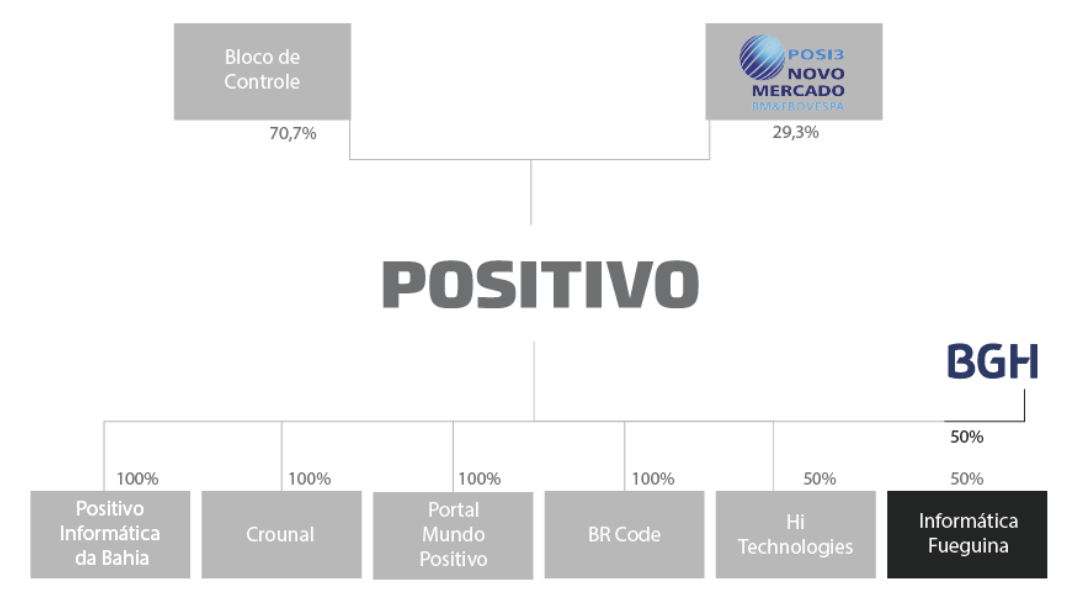
\includegraphics[width=1.0\textwidth]{Img/Corporativo}
\caption{Figura que demonstra o domínio e capital social da \nomeCompletoPositivo{}.}
\par\end{centering}
\end{figure}

Em 2016, a Positivo Tecnologia foi uma das maiores fabricantes de computadores no Brasil, respondendo por 15,3\% do número total de computadores vendidos no mercado brasileiro, de acordo com a IDC. No mesmo período, obtiveram uma participação de 19,9\% do mercado de varejo. Uma parcela substancial da produção de computadores é vendida através de grandes redes de varejo, com as quais o grupo mantém sólido relacionamento comercial, em função principalmente dos preços competitivos, do reconhecimento da marca e assistência técnica.

Adicionalmente, a companhia atua no mercado argentino por meio da marca \nomePositivoAr{}, fruto de uma joint venture com um parceiro local. Em 2015, os computadores \nomePositivoAr{} atingiram uma participação de 9,5\%, segundo a IDC.

No Brasil, a Positivo Tecnologia oferece uma linha completa de dispositivos, incluindo computadores de mesa (desktops e all-in-ones), computadores portáteis (notebooks e netbooks) e tablets, que são produzidos em Manaus (AM). Em 2012, a Companhia ingressou no mercado de telefones celulares, com a oferta de smartphones e messaging phones.

\begin{figure}[h]
\begin{centering}
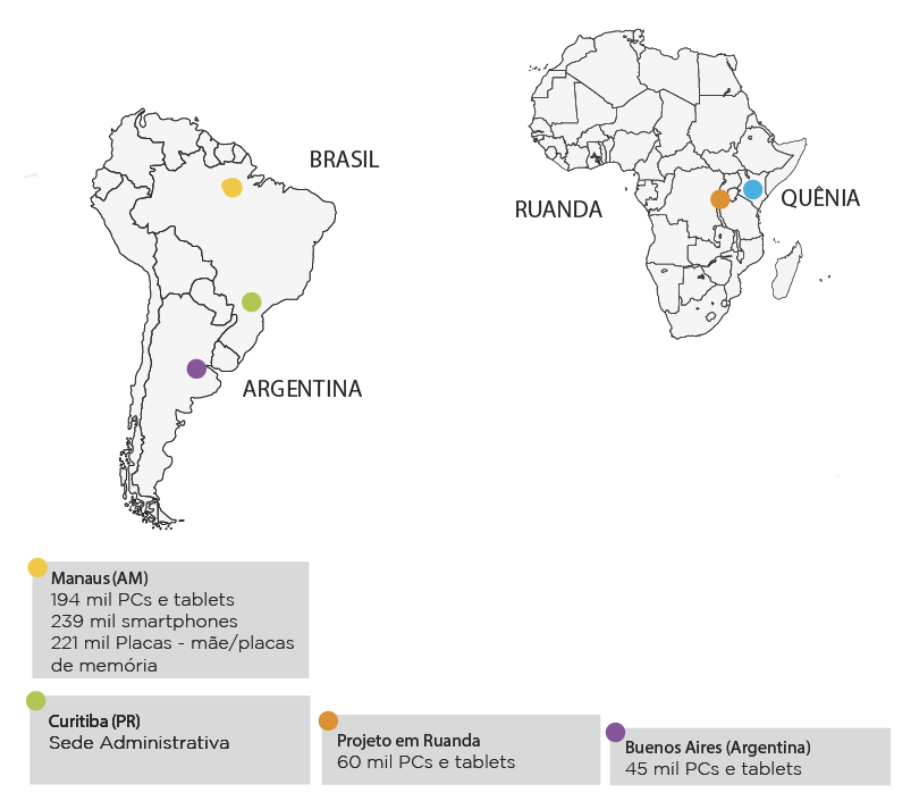
\includegraphics[width=1.0\textwidth]{Img/PositivoMundo}
\caption{Operações da \nomePositivo{} a nível mundial, bastante expressiva na América Latina e observa-se também sítios na África.}
\par\end{centering}
\end{figure}

Além disso, para atendimento e suporte aos milhões de consumidores finais, empresas e órgãos do governo, conta com uma ampla e capacitada rede de assistências técnicas cobrindo a totalidade do território nacional, e com a CRP - Central de Relacionamento Positivo, que registrou em média, 2,9 mil contatos diários em 2016. Grande parte destes contatos se refere a questões básicas sobre uso do computador, sistema operacional ou problemas com conexões, uma vez que muitos dos clientes estão adquirindo seu computador pela primeira vez.

Parcela menor da receita da Companhia provém do Segmento de Tecnologia Educacional, no qual acredita ser líder absoluto no País. A Companhia oferece soluções de infraestrutura e gestão, aplicativos e plataformas educacionais, portais de educação, além de formação de professores e acompanhamento pedagógico. Os portais têm mais de 1,2 milhões de usuários ativos, com modelo de receita recorrente mensal. 

As soluções educacionais da Positivo Tecnologia estão presentes em mais de 14 mil escolas e são exportadas para mais de 40 países. Dentre os principais produtos estão mesas educacionais, dispositivos móveis, lousas interativas, dispositivos de armazenamento e recarga, projetores, acess point, e sistema de gerenciamento de aulas. A Companhia é também distribuidor exclusivo no Brasil de empresas líderes no desenvolvimento e distribuição de software educacional, bem como distribui produtos da LEGO\texttrademark Education no território nacional.

Em 2016, a Companhia ingressou no mercado de tecnologia médica por meio da aquisição de 50\% do capital social da Hi Technologies S.A., empresa com forte foco em P\&D para a oferta de produtos inovadores em saúde.


\chapter[Exercício 1]{Exercício 1}
Utilizando o arquivo "Serie\_Dados.csv", realize as seguintes etapas:

\section{Crie a série temporal dos retornos Ln, ou seja, $r=\ln(\frac{P_{t+1}}{P_{t}})$}

\inputminted{R}{Src/R/ex1a.R}

\section{Para cada ação construa o histograma dos retornos. Comente o resultado dos histogramas, verifique também o desvio padrão e a média de cada série.}

\begin{center}
\begin{centering}
\includegraphics[width=0.95\textwidth]{dist1b}
\par\end{centering}
%\caption{\label{fig:PlotAcf4a}Plot Acf}
\par\end{center}

Percebe-se que todas as variáveis apresentam distribuição normal após a transformação das séries temporais por logaritmo neperiano. No caso da variável DOLAR, apresenta-se uma homogeneidade maior em comparação com as demais variáveis.

% Preview source code for paragraph 0

\begin{center}
\begin{tabular}{c|c|c}
\hline 
 & Média & Desv Padrão\tabularnewline
\hline 
VALE5 & 0.00013 & 0.01839\tabularnewline
\hline 
GOLL4 & -0.00049 & 0.03248\tabularnewline
\hline 
AMBV4 & 0.00127 & 0.01426\tabularnewline
\hline 
ITUB4 & -0.00003 & 0.01833\tabularnewline
\hline 
BBDC4 & 0.00021 & 0.01709\tabularnewline
\hline 
BVMF3 & 0.00009 & 0.02194\tabularnewline
\hline 
RAPT4 & 0.00035 & 0.02012\tabularnewline
\hline 
MYPK3 & 0.00102 & 0.02256\tabularnewline
\hline 
GOAU4 & -0.00020 & 0.02253\tabularnewline
\hline 
LLXL3 & -0.00122 & 0.04117\tabularnewline
\hline 
CSAN3 & 0.00088 & 0.01928\tabularnewline
\hline 
DOLAR & 0.00025 & 0.00772\tabularnewline
\hline 
\end{tabular}
\par\end{center}


% imagem
\section{Calcule o ACF e PACF de cada série de retornos. Comente os resultados.}

\begin{center}
\begin{centering}
\includegraphics[width=0.95\textwidth]{dist1c_acf_pac}
\par\end{centering}
%\caption{\label{fig:PlotAcf4a}Plot Acf}
\par\end{center}

Utilizando-se as séries de dados transformadas pelo LN, percebeu-se, através do cálculo da Autocorrelação (ACF) que todas as séries são estacionárias. Em complemento da análise, podemos concluir que todos as Autocorrelações Parciais (PACF) possuem pouca defasagem.


\chapter[Exercício 2]{Exercício 2}
Para cada um dos processos abaixo gere 200 observações. Faça um gráfico da série, ACF e PACF. Comente os resultados.

\section{Série aleatória, observações iid da distribuição N(0,1)}

% Comments 

\begin{center}
\begin{centering}
\includegraphics[width=0.95\textwidth]{dist2d_plot_ts}
\par\end{centering}
%\caption{\label{fig:PlotAcf4a}Plot Acf}
\par\end{center}

\begin{center}
\begin{centering}
\includegraphics[width=0.95\textwidth]{dist2d_acf}
\par\end{centering}
%\caption{\label{fig:PlotAcf4a}Plot Acf}
\par\end{center}

\begin{center}
\begin{centering}
\includegraphics[width=0.95\textwidth]{dist2d_pacf}
\par\end{centering}
%\caption{\label{fig:PlotAcf4a}Plot Acf}
\par\end{center}

Para a distribuição N(0,1) os resultados apresentam uma série estacionária com pouca sazonalidade vista no gráfico e acrescentada na análise do ACF, pois quase todos pontos se mantém dentro das bandas de defasagem. O único ponto que apresenta defasagem no PACF é o ponto 16.

%\subsection{Código Fonte}

%\inputminted{R}{Src/R/ex2d.R}

\section{Série com tendência estocástica $x_{i}=x_{t-1}+N(1,5^{2})$.}

\begin{center}
\begin{centering}
\includegraphics[width=0.95\textwidth]{dist2e_plot_ts}
\par\end{centering}
%\caption{\label{fig:PlotAcf4a}Plot Acf}
\par\end{center}

\begin{center}
\begin{centering}
\includegraphics[width=0.95\textwidth]{dist2e_acf}
\par\end{centering}
%\caption{\label{fig:PlotAcf4a}Plot Acf}
\par\end{center}

\begin{center}
\begin{centering}
\includegraphics[width=0.95\textwidth]{dist2e_pacf}
\par\end{centering}
%\caption{\label{fig:PlotAcf4a}Plot Acf}
\par\end{center}

No caso da tendência estocástica os resultados apresentam uma série não estacionária com pouca sazonalidade vista na linha de tendência no gráfico, porém ao analisar o gráfico apresentado após o cálculo da Autocorrelação (ACF), verifica-se que na verdade é uma série estacionária pois os pontos de defasagem tendem a zero.

%\subsection{Código Fonte}

%\inputminted{R}{Src/R/ex2e.R}

%\subsection{Saída}

\section{Série com correlação de curto-prazo, $x_{i}=0.95x_{t-1}+N(0,1)$.}

\begin{center}
\begin{centering}
\includegraphics[width=0.95\textwidth]{dist2f_plot_ts}
\par\end{centering}
%\caption{\label{fig:PlotAcf4a}Plot Acf}
\par\end{center}

\begin{center}
\begin{centering}
\includegraphics[width=0.95\textwidth]{dist2f_acf}
\par\end{centering}
%\caption{\label{fig:PlotAcf4a}Plot Acf}
\par\end{center}

\begin{center}
\begin{centering}
\includegraphics[width=0.95\textwidth]{dist2f_pacf}
\par\end{centering}
%\caption{\label{fig:PlotAcf4a}Plot Acf}
\par\end{center}

Na análise da correlação de curto-prazo pode-se concluir que é uma série estacionária pois em todas os gráficos os pontos tendem a zero.

%\subsection{Código Fonte}
%\inputminted{R}{Src/R/ex2f.R}

\section{Série com correlações negativas, $x_{i}=-0.95x_{t-1}+N(0,1)$.}

\begin{center}
\begin{centering}
\includegraphics[width=0.95\textwidth]{dist2g_plot_ts}
\par\end{centering}
%\caption{\label{fig:PlotAcf4a}Plot Acf}
\par\end{center}

\begin{center}
\begin{centering}
\includegraphics[width=0.95\textwidth]{dist2g_acf}
\par\end{centering}
%\caption{\label{fig:PlotAcf4a}Plot Acf}
\par\end{center}

\begin{center}
\begin{centering}
\includegraphics[width=0.95\textwidth]{dist2g_pacf}
\par\end{centering}
%\caption{\label{fig:PlotAcf4a}Plot Acf}
\par\end{center}


%\subsection{Código Fonte}
%\inputminted{R}{Src/R/ex2g.R}
Na série de correlações negativas     conclui-se que é estacionária e é interessante nota que no ACF e PACF há pontos de defasagens negativos.

\section{Médias móveis, $x_{t}=\epsilon_{t}+0,6\epsilon_{t-1}$ e $\epsilon_{t}\sim N(0,1)$}

\begin{center}
\begin{centering}
\includegraphics[width=0.95\textwidth]{dist2h_plot_ts}
\par\end{centering}
%\caption{\label{fig:PlotAcf4a}Plot Acf}
\par\end{center}

\begin{center}
\begin{centering}
\includegraphics[width=0.95\textwidth]{dist2h_acf}
\par\end{centering}
%\caption{\label{fig:PlotAcf4a}Plot Acf}
\par\end{center}

\begin{center}
\begin{centering}
\includegraphics[width=0.95\textwidth]{dist2h_pacf}
\par\end{centering}
%\caption{\label{fig:PlotAcf4a}Plot Acf}
\par\end{center}

Na série de médias móveis conclui-se que é estacionária e como no caso anterior vale a observação que neste caso apresentam-se pontos de defasagem tanto para o lado positivo quanto para o lado negativo.

%\subsection{Código Fonte}
%\inputminted{R}{Src/R/ex2h.R}


\chapter[Exercício 3]{Exercício 3}
Utilize a série abaixo para resolver cada item.

\emph{An example of a time series that can probably be described using an additive model with a trend and no seasonality is the time series of the annual diameter of women’s skirts at the hem, from 1866 to 1911. The data is available in the \href{http://robjhyndman.com/tsdldata/roberts/skirts.dat}{web file}} (original data from Hipel and McLeod, 1994).

%a
\section{\label{sec:3a} Faça a leitura da série de dados e os tratamentos necessários para considerar a mesma como uma série temporal}

\inputminted{R}{Src/R/ex3a.R}

%b
\section{Faça a decomposição da série do item anterior: Sazonalidade, Tendência e Aleatória.}
Não há sazonalidade nesta séries de dados, muito menos flutuações randômicas. Decompondo, séries não sazonais, retirando-se as flutuações randômicas para ficar claro a tendência, o que pode ser notado é que a \emph{Série Original}, sem transformação, já apresenta uma tendência de alta nos 15 primeiros anos e entra em tendência de queda.

\begin{center}
\begin{centering}
\includegraphics[width=0.95\textwidth]{dist3a_plot_ts}
\par\end{centering}
%\caption{\label{fig:PlotAcf4a}Plot Acf}
\par\end{center}

\begin{center}
\begin{centering}
\includegraphics[width=0.95\textwidth]{dist3b_plot_ts_ma3}
\par\end{centering}
%\caption{\label{fig:PlotAcf4a}Plot Acf}
\par\end{center}



\chapter[Exercício 4]{Exercício 4}
Usando a função arima.sim gere as seguintes simulações (300 ptos).

Para cada simulação, plote o gráfico da série, calcule o ACF e PACF. Usando estes resultados conclua como deve ser o comportamento da ACF de PACF de um modelo autoregressivo( AR.)

\section{Processo AR(1) onde $\theta_{0}=0$, $\theta_{1}=0.7$}

\begin{center}
%\begin{figure}[h]
\begin{centering}
\includegraphics[width=0.95\textwidth]{dist4a_plot_ts}
\par\end{centering}
%\caption{\label{fig:PlotAcf4a}Plot Acf}
%\end{figure}
%\vspace*{-40pt}
\par\end{center}


\begin{center}
%\begin{figure}[h]
\begin{centering}
\includegraphics[width=0.95\textwidth]{dist4a_plot_acf}
\par\end{centering}
%\caption{\label{fig:PlotAcf4a}Plot Acf}
%\end{figure}
%\vspace*{-40pt}
\par\end{center}

\begin{center}
%\begin{figure}[h]
\begin{centering}
\includegraphics[width=0.95\textwidth]{dist4a_plot_pacf}
\par\end{centering}
%\caption{\label{fig:PlotAcf4a}Plot Acf}
%\end{figure}
%\vspace*{-40pt}
\par\end{center}



\section{Processo AR(1) onde $\theta_{0}=0$, $\theta_{1}=-0.7$}

\begin{center}
%\begin{figure}[h]
\begin{centering}
\includegraphics[width=0.95\textwidth]{dist4b_plot_ts}
\par\end{centering}
%\caption{\label{fig:PlotAcf4a}Plot Acf}
%\end{figure}
%\vspace*{-40pt}
\par\end{center}


\begin{center}
%\begin{figure}[h]
\begin{centering}
\includegraphics[width=0.95\textwidth]{dist4b_plot_acf}
\par\end{centering}
%\caption{\label{fig:PlotAcf4a}Plot Acf}
%\end{figure}
%\vspace*{-40pt}
\par\end{center}

\begin{center}
%\begin{figure}[h]
\begin{centering}
\includegraphics[width=0.95\textwidth]{dist4b_plot_pacf}
\par\end{centering}
%\caption{\label{fig:PlotAcf4a}Plot Acf}
%\end{figure}
%\vspace*{-40pt}
\par\end{center}



\section{Processo AR(2) onde $\theta_{0}=0$, $\theta_{1}=-0.3$ e $\theta_{2}=0.5$}

\begin{center}
%\begin{figure}[h]
\begin{centering}
\includegraphics[width=0.95\textwidth]{dist4c_plot_ts}
\par\end{centering}
%\caption{\label{fig:PlotAcf4a}Plot Acf}
%\end{figure}
%\vspace*{-40pt}
\par\end{center}


\begin{center}
%\begin{figure}[h]
\begin{centering}
\includegraphics[width=0.95\textwidth]{dist4c_plot_acf}
\par\end{centering}
%\caption{\label{fig:PlotAcf4a}Plot Acf}
%\end{figure}
%\vspace*{-40pt}
\par\end{center}

\begin{center}
%\begin{figure}[h]
\begin{centering}
\includegraphics[width=0.95\textwidth]{dist4c_plot_pacf}
\par\end{centering}
%\caption{\label{fig:PlotAcf4a}Plot Acf}
%\end{figure}
%\vspace*{-40pt}
\par\end{center}


\section{Processo MA(1) onde $\theta_{0}=0$, $\theta_{1}=0.6$}

\begin{center}
%\begin{figure}[h]
\begin{centering}
\includegraphics[width=0.95\textwidth]{dist4d_plot_ts}
\par\end{centering}
%\caption{\label{fig:PlotAcf4a}Plot Acf}
%\end{figure}
%\vspace*{-40pt}
\par\end{center}


\begin{center}
%\begin{figure}[h]
\begin{centering}
\includegraphics[width=0.95\textwidth]{dist4d_plot_acf}
\par\end{centering}
%\caption{\label{fig:PlotAcf4a}Plot Acf}
%\end{figure}
%\vspace*{-40pt}
\par\end{center}

\begin{center}
%\begin{figure}[h]
\begin{centering}
\includegraphics[width=0.95\textwidth]{dist4d_plot_pacf}
\par\end{centering}
%\caption{\label{fig:PlotAcf4a}Plot Acf}
%\end{figure}
%\vspace*{-40pt}
\par\end{center}

\section{Processo MA(1) onde $\theta_{0}=0$, $\theta_{1}=-0.6$}

\begin{center}
%\begin{figure}[h]
\begin{centering}
\includegraphics[width=0.95\textwidth]{dist4e_plot_ts}
\par\end{centering}
%\caption{\label{fig:PlotAcf4a}Plot Acf}
%\end{figure}
%\vspace*{-40pt}
\par\end{center}


\begin{center}
%\begin{figure}[h]
\begin{centering}
\includegraphics[width=0.95\textwidth]{dist4e_plot_acf}
\par\end{centering}
%\caption{\label{fig:PlotAcf4a}Plot Acf}
%\end{figure}
%\vspace*{-40pt}
\par\end{center}

\begin{center}
%\begin{figure}[h]
\begin{centering}
\includegraphics[width=0.95\textwidth]{dist4e_plot_pacf}
\par\end{centering}
%\caption{\label{fig:PlotAcf4a}Plot Acf}
%\end{figure}
%\vspace*{-40pt}
\par\end{center}

Em análise aos resultados vistos nos gráficos pode-se concluir que o processo do modelo auto regressivo (AR) possuem ACF  infinita com queda exponencial e o PACF igual a zero para a maioria das defasagens.


\chapter[Exercício 5]{Exercício 5}
Obtenha a série histórica do PIB Brasil no site \href{http://www.bcb.gov.br/pre/portalCidadao/cadsis/series.asp?idpai=PORTALBCB}{portal do cidadão}.

Código da série: 1232

\section{Plote o gráfico da série usando o R}

\begin{center}
\begin{centering}
\includegraphics[width=0.95\textwidth]{dist5a_plot_ts}
\par\end{centering}
%\caption{\label{fig:PlotAcf4a}Plot Acf}
\par\end{center}

\section{Faça a decomposição da série em: Sazonalidade, Tendência e Aleatória.}

\begin{center}
\begin{centering}
\includegraphics[width=0.95\textwidth]{dist5b_decompose}
\par\end{centering}
%\caption{\label{fig:PlotAcf4a}Plot Acf}
\par\end{center}




% ----------------------------------------------------------
% Finaliza a parte no bookmark do PDF
% para que se inicie o bookmark na raiz
% e adiciona espaço de parte no Sumário
% ----------------------------------------------------------
\phantompart

% ---
% Conclusão - Recomendação de qual protótipo
% ---
%\chapter{Conclusões}
% ---

%Placeholder
%\label{chap:conclusao}

\begin{figure}
\begin{centering}
\subfloat[\label{fig:prototipo-familia}Conforto,
espaço e filhos.]{\begin{centering}
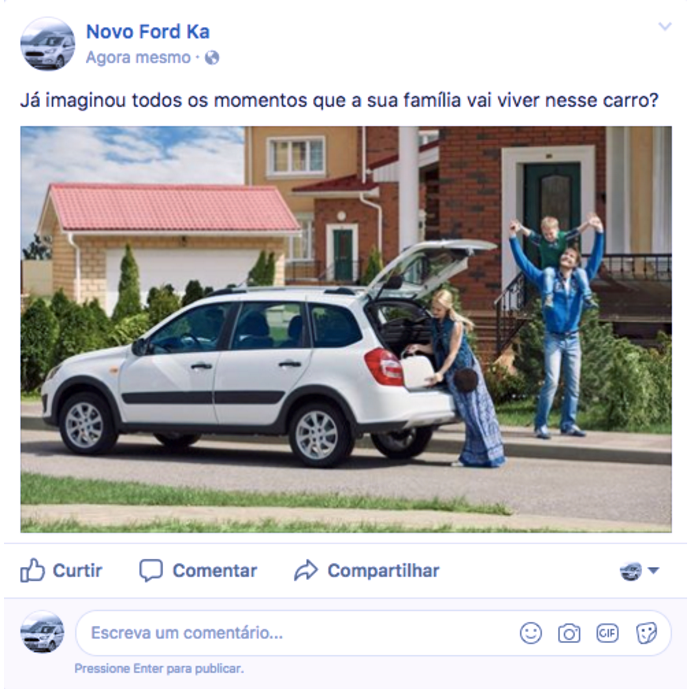
\includegraphics[height=0.30\textheight]{Imagens/p1_familia}~~
\par\end{centering}
}\subfloat[\label{fig:prototipo-versatil}Aborda o efeito versátil do carro.]{\begin{centering}
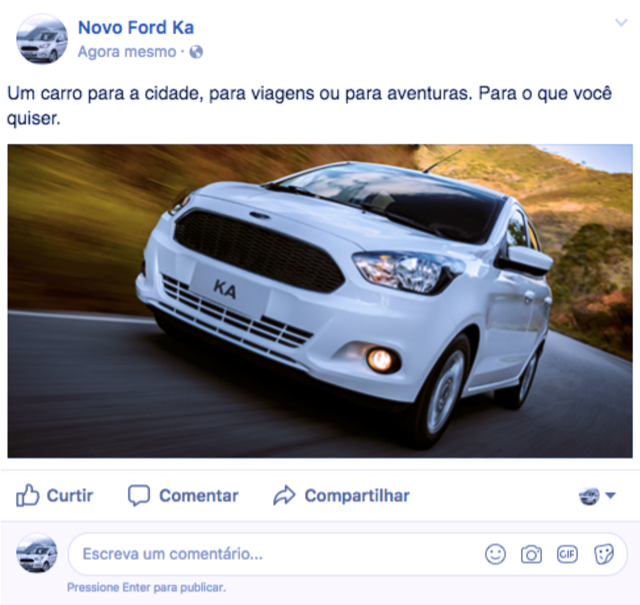
\includegraphics[height=0.30\textheight]{Imagens/p1_prototipo}
\par\end{centering}
}
\par\end{centering}
\caption{Peças ilustrativas de uma campanha em formato carrossel.}
\end{figure}

De acordo com o desenvolvido no capítulo \ref{chap:analise}, com
as tabelas \ref{tab:prototipo-vs-cluster} e \ref{tab:prototipo-analise},
contrasta a homogeneidade dos protótipo 2 e 3 à heterogeneidade do
protótipo 1. À primeira vista, percebe-se que os três protótipos possuem
proporções da população muito parecidas, entretanto há uma grande
diferença entre o protótipo 1, heterogêneo, com os demais protótipos.
Isto é, a possibilidade de uma campanha publicitária informativa unida
a transformativas que possibilitarão, se escolhido o protótipo 1,
abranger também os clusters \nomeCc{} e \nomeCb{}, dado que pela
própria heterogeneidade do protótipo 1, certas propagandas que apelam
para determinadas características do protótipo podem aumentar a aceitação
de uma campanha baseada neste protótipo.

\begin{table}
\begin{centering}
\begin{tabular}{c|>{\centering}p{0.28\textwidth}|>{\centering}p{0.28\textwidth}|>{\centering}p{0.28\textwidth}}
\hline 
 & Protótipo 1 & Protótipo 2 & Protótipo 3\tabularnewline
\hline 
Bom & Preferido entre \nomeCa{} e \nomeCd{}. & Amplamente preferido pelo cluster dos \nomeCc{}. & Amplamente preferido pelos \nomeCb{}, focados em Imagem.\tabularnewline
\hline 
Ruim & Somente uma estratégia de marketing não é suficiente, dada a sua heterogeneidade
e várias afinidades. & Difícil para a publicidade porque se mostra indiferente a carros.
Importam-se apenas com o preço. & Uma campanha publicitária em Imagem somente não gera interesse de
outros clusters.\tabularnewline
\hline 
\end{tabular}
\par\end{centering}
\caption{\label{tab:prototipo-analise}Vantagens e desvantagens por protótipos.}
\end{table}


Por exemplo, se uma campanha publicitária apelar de maneira informativa
e transformativa para os aspectos de Imagem e Utilitário do carro,
é possível abranger os clusters mencionados anteriormente, sustentando
assim uma aceitação maior por parte da população. Ou seja, escolhe-se
a versatilidade do protótipo 1, numa eventual campanha publicitária
como elemento.

\begin{figure}
\begin{centering}
\subfloat[\label{fig:painel-cambio}Acabamento e câmbio.]{\begin{centering}
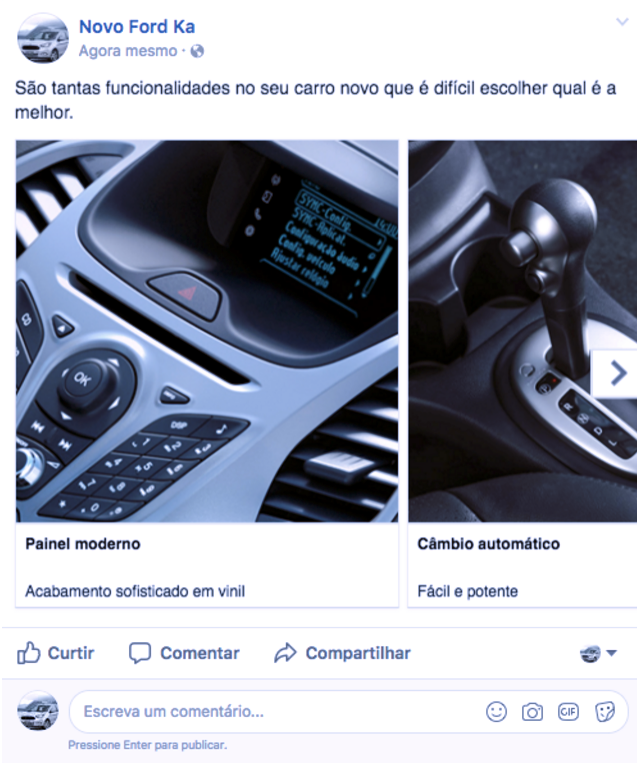
\includegraphics[height=0.34\textheight]{Imagens/p1_interior}
\par\end{centering}
}~~\subfloat[\label{fig:ar}Ar-condicionado.]{\begin{centering}
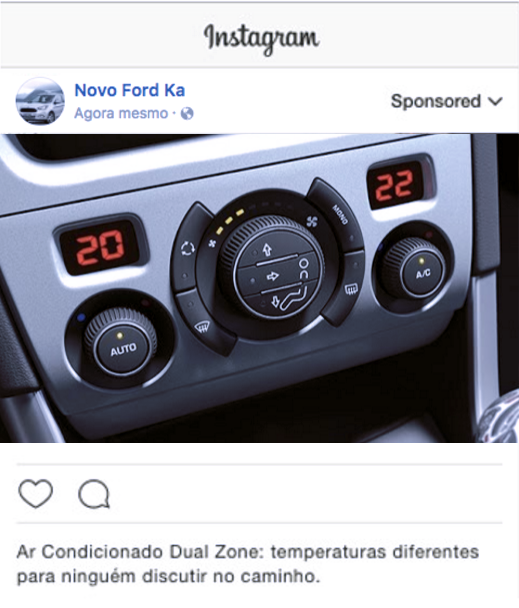
\includegraphics[height=0.34\textheight]{Imagens/p1_interior_painel}
\par\end{centering}
}
\par\end{centering}
\caption{Peças multifuncionais para Utilitário e Imagem.}
\end{figure}


\section{Recomendações para Campanha Publicitária}

Com base nas características analisadas dos grupos \nomeCa{} e \nomeCd{}
será feita uma combinação de campanhas publicitárias: para os \nomeCa{},
uma campanha transformativa mesclando os três atributos: Imagem, Utilitário
e Preço. Para os \nomeCd{}, uma campanha ressaltando o carro como
utilitário. Por se tratar de dois grupos diferentes vamos destacar
multifuncionalidade, tecnologia, versatilidade e conforto.

É possível uma campanh que foque nas seguintes características: confortável
e espaçoso. O público-alvo seriam os \nomeCd{} que preferem carros
como bens utilitários, destacando o porta-malas espaçoso para a família.
Os \nomeCd{} são formados predominantemente por mulheres com filhos,
por isso o destaque a família, na figura \ref{fig:prototipo-familia}.

A campanha com formato em carrossel irá abordar a característica de
multifuncionalidade. A publicidade tem foco nos \nomeCa{} combinando
funcionalidades (Utilitário) que valorizem o carro (Preço) e que tragam
mais sofisticação (Imagem), como vê-se nas figuras \ref{fig:painel-cambio}
e \ref{fig:ar}.

Finalmente, a figura \ref{fig:prototipo-versatil} seria veiculada
em formato vídeo, tanto em Facebook quanto na televisão. Destaca a
versatilidade do Ford Ka\texttrademark, valorizando o fato de ser
um carro potente (Utilitário) e ainda assim econômico (Preço). Em
televisão, dá-se preferência é por intervalos de jogos de futebol
buscando atingir um público predominantemente masculino que gosta
de esportes e aventuras. 



% ----------------------------------------------------------
% ELEMENTOS PÓS-TEXTUAIS
% ----------------------------------------------------------
\postextual
% ----------------------------------------------------------

% ----------------------------------------------------------
% Referências bibliográficas
% ----------------------------------------------------------
%\bibliography{referencias}

% ----------------------------------------------------------
% Glossário
% ----------------------------------------------------------
%
% Consulte o manual da classe abntex2 para orientações sobre o glossário.
%
%\glossary

% ----------------------------------------------------------
% Apêndices
% ----------------------------------------------------------

% ---
% Inicia os apêndices
% ---
%\begin{apendicesenv}

%% Imprime uma página indicando o início dos apêndices
%\partapendices

%% ----------------------------------------------------------
%\chapter{Quisque libero justo}
%% ----------------------------------------------------------

%\lipsum[50]

%% ----------------------------------------------------------
%\chapter{Nullam elementum urna vel imperdiet sodales elit ipsum pharetra ligula
%ac pretium ante justo a nulla curabitur tristique arcu eu metus}
%% ----------------------------------------------------------
%\lipsum[55-57]

%\end{apendicesenv}
% ---


% ----------------------------------------------------------
% Anexos
% ----------------------------------------------------------

% ---
% Inicia os anexos
% ---
\begin{anexosenv}

%% Imprime uma página indicando o início dos anexos
\partanexos

\chapter[Código Fonte]{Código Fonte}
\inputminted{R}{Src/R/exercicios.R}


%% ---
%\chapter{Morbi ultrices rutrum lorem.}
%% ---
%\lipsum[30]

%% ---
%\chapter{Cras non urna sed feugiat cum sociis natoque penatibus et magnis dis
%parturient montes nascetur ridiculus mus}
%% ---

%\lipsum[31]

%% ---
%\chapter{Fusce facilisis lacinia dui}
%% ---

%\lipsum[32]

\end{anexosenv}

%---------------------------------------------------------------------
% INDICE REMISSIVO
%---------------------------------------------------------------------
\phantompart
\printindex
%---------------------------------------------------------------------

\end{document}
